% Manual for K
% (c) 2003, 2007 Douglas G. Scofield, dgscofie@indiana.edu
% 

\documentclass[12pt,twoside,letterpaper,fleqn]{report}
\pagestyle{headings}      % headings only, which is fine
\topmargin -0.5in         % one inch less than top edge of paper to top of head
\headsep 0.5in            % distance b/w head and body of page
\oddsidemargin 0.25in     % one inch less than left edge to margin on RH pages
\evensidemargin 0in       % one inch less than right edge to margin on LH pages
\textwidth 6.25in         % normal width of text on a page
\textheight 8.5in         % normal height of the body of a page
% \parskip 15pt       %7.2pt    % sets spacing between paragraphs
% \parindent 0pt		  % sets leading space for paragraphs
%
\usepackage{marvosym}  % \Male and \Female symbols
\usepackage{topcapt}
\usepackage{epigraph}  % to typeset epigraphs
  \renewcommand{\epigraphsize}{\footnotesize}
\usepackage{url}       % to specify URLs throughout the document, in ltxmisc download
\usepackage{natbib}
    \bibliographystyle{authordatedgs}
    \bibpunct{(}{)}{;}{a}{}{,}
\usepackage{amsmath}      % AMS math macros
	\numberwithin{equation}{section}  % equation numbering
	\DeclareMathOperator{\abs}{abs}
\usepackage{graphicx}     % for handling EPS etc.
\usepackage{lscape}
\usepackage{setspace}
\usepackage{longtable}    % for tables that span more than one page
	\setcounter{LTchunksize}{100}  % for the longtable package
\usepackage{verbatim}     % for \begin{comment} \end{comment}
\usepackage{setspace}     % for singlespacing and doublespacing
\usepackage{listings}     % for including source code
	\lstset{                  % parameters to be used for source code listing
		language=C,
		basicstyle=\small\ttfamily,
		commentstyle=\small\ttfamily,
		basewidth=0.5em,
		lineskip=-0.2pt,
		xleftmargin=0.5in,
    	float=[h],
    	aboveskip=\bigskipamount,
    	belowskip=\bigskipamount,
		mathescape=true}
\usepackage{fancyvrb}
    \DefineVerbatimEnvironment{ROutput}{Verbatim}
        {fontfamily=tt,
         fontsize=\small,
         baselinestretch=1,
         xleftmargin=0.5in,
         frame=none,
         numbers=none,
        }
\usepackage{listings}  % for including long-form C source code
    \lstnewenvironment{Clong}[1][]
        {\lstset{
            language=C,
            basicstyle=\small\ttfamily,
            commentstyle=\small\normalfont\itshape,%commentstyle=\small\ttfamily,
            breaklines=true,
            basewidth=0.5em,
            lineskip=-0.2pt,
            xleftmargin=0in,
            aboveskip=\bigskipamount,
            belowskip=\bigskipamount,
            mathescape=true,
            escapechar=|,
            #1
        }}
    {}
    \lstnewenvironment{C}[1][]
        {\lstset{
            language=C,
            basicstyle=\small\ttfamily,
            commentstyle=\small\normalfont\itshape,%commentstyle=\small\ttfamily,
            breaklines=true,
            basewidth=0.5em,
            lineskip=-0.2pt,
            xleftmargin=0.5in,
            aboveskip=\bigskipamount,
            belowskip=\bigskipamount,
            mathescape=true,
            escapechar=|,
            #1
        }}
    {}
    \lstnewenvironment{R}[1][]
        {\lstset{
            language=R,
            basicstyle=\small\ttfamily,
            commentstyle=\small\normalfont\itshape,%commentstyle=\small\ttfamily,
            breaklines=true,
            basewidth=0.5em,
            lineskip=-0.2pt,
            xleftmargin=0.5in,
            aboveskip=\bigskipamount,
            belowskip=\bigskipamount,
            mathescape=true,
            #1
        }}
    {}
    \lstnewenvironment{Matlab}[1][]
        {\lstset{
            language=Matlab,
            basicstyle=\small\ttfamily,
            commentstyle=\small\normalfont\itshape,%commentstyle=\small\ttfamily,
            breaklines=true,
            basewidth=0.5em,
            lineskip=-0.2pt,
            xleftmargin=0.25in,
            aboveskip=\bigskipamount,
            belowskip=\bigskipamount,
            mathescape=true,
            #1
        }}
    {}


%%%%%% Macros
%
%
%
\newcommand{\REDO}{{\bf {\em REDO!}}}
\newcommand{\K}{{\bf K}}
\newcommand{\ProbDist}[2]{\mbox{{#1}$(#2)$}}
\newcommand{\Order}[1]{\mbox{$\text{{\bf O}}(#1)$}}  % the O() expressions of algorithm time
\newcommand{\genotype}[2]{\mbox{$({#1}{#2})$}}
% This generates a code fragment
% \newcommand{\Kcode}[1]{\mbox{{\tt #1}}}
\newcommand{\Kcode}[1]{{\tt #1}}
% This generates command-line-style entries
\newcommand{\Cmdline}[1]{{\tt #1}}
% These generate \tt-style code for a KConfig member access: K->#1[#2][#3][#4]
\newcommand{\KK}{\mbox{{\tt K}}}  % the name of the 'master' KConfig
\newcommand{\KKN}{\mbox{{\tt KN}}}  % the name of the 'master' KConfig_n
\newcommand{\Kmember}[1]{\mbox{{\tt K->#1}}}
\newcommand{\Kmemberi}[2]{\mbox{{\tt K->#1[{\it #2}\/]}}}
\newcommand{\Kmemberij}[3]{\mbox{{\tt K->#1[{\it #2}\/][{\it #3}\/]}}}
\newcommand{\Kmemberijk}[4]{\mbox{{\tt K->#1[{\it #2}\/][{\it #3}\/][{\it #4}\/]}}}
\newcommand{\KScalar}{\mbox{\tt KScalar}}
\newcommand{\KInt}{\mbox{\tt KInt}}
\newcommand{\KArray}{\mbox{\tt KArray}}
\newcommand{\KConfig}{\mbox{\tt KConfig}}
\newcommand{\KConfign}{\mbox{\tt KConfig\_n}}

\newcommand{\izero}{\mbox{$i_0$\/}}
\newcommand{\jzero}{\mbox{$j_0$\/}}
\newcommand{\ione}{\mbox{$i_1$\/}}
\newcommand{\jone}{\mbox{$j_1$\/}}
\newcommand{\nzero}{\mbox{$n_0$\/}}
\newcommand{\none}{\mbox{$n_1$\/}}
\newcommand{\Lijij}{\mbox{$L_{i_0\/,j_0\/,i_1\/,j_1\/}$}}
\newcommand{\Lijzero}{\mbox{$L_{i_0\/,j_0\/}$}}
\newcommand{\Lijone}{\mbox{$L_{i_1\/,j_1\/}$}}
\newcommand{\Mizero}{\mbox{$M_{i_0}$\/}}
\newcommand{\Mjzero}{\mbox{$M_{j_0}$\/}}
\newcommand{\Mione}{\mbox{$M_{i_1}$\/}}
\newcommand{\Mjone}{\mbox{$M_{j_1}$\/}}
\newcommand{\wnested}{\mbox{$\omega_{i_0\/,j_0\/,i_1\/,j_1\/}$}}
\newcommand{\meanwnested}{\mbox{$\bar{\omega}_{01}$}}

\newcommand{\gami}{\mbox{$f_{i}$}}
\newcommand{\gammalei}{\mbox{$f_{i}^{\text{\Male}}$}}
\newcommand{\gamfemalei}{\mbox{$f_{i}^{\text{\Female}}$}}
\newcommand{\gammalek}{\mbox{$f_{k}^{\text{\Male}}$}}
\newcommand{\gamfemalek}{\mbox{$f_{k}^{\text{\Female}}$}}
\newcommand{\gammaleik}{\mbox{$f_{i-k}^{\text{\Male}}$}}
\newcommand{\gamfemaleik}{\mbox{$f_{i-k}^{\text{\Female}}$}}

\newcommand{\gamii}{\mbox{$f_{i_0,i_1}$}}
\newcommand{\gammaleii}{\mbox{$f_{i_0,i_1}^{\text{\Male}}$}}
\newcommand{\gamfemaleii}{\mbox{$f_{i_0,i_1}^{\text{\Female}}$}}
\newcommand{\gammalekk}{\mbox{$f_{k_0,k_1}^{\text{\Male}}$}}
\newcommand{\gamfemalekk}{\mbox{$f_{k_0,k_1}^{\text{\Female}}$}}
\newcommand{\gammaleikik}{\mbox{$f_{i_0-k_0,i_1-k_1}^{\text{\Male}}$}}
\newcommand{\gamfemaleikik}{\mbox{$f_{i_0-k_0,i_1-k_1}^{\text{\Female}}$}}
\newcommand{\gammalekik}{\mbox{$f_{k_0,i_1-k_1}^{\text{\Male}}$}}
\newcommand{\gamfemalekik}{\mbox{$f_{k_0,i_1-k_1}^{\text{\Female}}$}}
\newcommand{\gammaleikk}{\mbox{$f_{i_0-k_0,k_1}^{\text{\Male}}$}}
\newcommand{\gamfemaleikk}{\mbox{$f_{i_0-k_0,k_1}^{\text{\Female}}$}}

\newcommand{\Mi}{\mbox{$M_{i}$}}
\newcommand{\Mj}{\mbox{$M_{j}$}}
\newcommand{\Mg}{\mbox{$M_{\gamma}$}}
\newcommand{\xijg}{\mbox{$x_{i,j}(\gamma)$}}
\newcommand{\xnjg}{\mbox{$x_{n,j}(\gamma)$}}
\newcommand{\xijgprev}{\mbox{$x_{(\text{prev})i,j}(\gamma)$}}
\newcommand{\xijij}{\mbox{$x_{i_0\/,j_0\/,i_1\/,j_1\/}$}}
\newcommand{\xpijg}{\mbox{$x'_{i,j}(\gamma)$}}
\newcommand{\xpijx}{\mbox{$x'_{i,j}(\xi)$}}
\newcommand{\xpij}{\mbox{$x'_{i,j}$}}
\newcommand{\xpnv}{\mbox{$x'_{n,v}$}}
\newcommand{\xpijij}{\mbox{$x'_{i_0\/,j_0\/,i_1\/,j_1\/}$}}
\newcommand{\xpnvnv}{\mbox{$x'_{n_0\/,v_0\/,n_1\/,v_1\/}$}}
\newcommand{\xppsijg}{\mbox{$x''_{(S)i,j}(\gamma)$}}
\newcommand{\xppaijg}{\mbox{$x''_{(A)i,j}(\gamma)$}}
\newcommand{\xppoig}{\mbox{$x''_{(O)i}(\gamma)$}}
\newcommand{\xppoijg}{\xppoig}
\newcommand{\xppijg}{\mbox{$x''_{i,j}(\gamma)$}}
\newcommand{\xppij}{\mbox{$x''_{i,j}$}}
\newcommand{\xppsijij}{\mbox{$x''_{(S)i_0\/,j_0\/,i_1\/,j_1\/}$}}
\newcommand{\xppaijij}{\mbox{$x''_{(A)i_0\/,j_0\/,i_1\/,j_1\/}$}}
\newcommand{\xppoii}{\mbox{$x''_{(O)i_0\/,i_1\/}$}}
\newcommand{\xppijij}{\mbox{$x''_{i_0\/,j_0\/,i_1\/,j_1\/}$}}
\newcommand{\Xijij}{\mbox{$X_{i_0\/,j_0\/,i_1\/,j_1\/}$}}
\newcommand{\Xijg}{\mbox{$X_{i,j}(\gamma)$}}
\newcommand{\Xij}{\mbox{$X_{i,j}$}}
\newcommand{\xij}{\mbox{$x_{i,j}$}}
\newcommand{\Lij}{\mbox{$L_{i,j}$}}              %  L(i,j)   load class across genotypes
\newcommand{\LCG}[3]{\mbox{$L(#1,#2;#3$)}}
\newcommand{\Lgij}{\mbox{$L_{i,j}(\gamma)$}}     %  L(i,j;g) load class by genotype
\newcommand{\Lijg}{\mbox{$L_{i,j}(\gamma)$}}     %  L(i,j;g) load class by genotype
\newcommand{\Lnv}{\mbox{$L_{n,v}$}}              %  L(n,v)   load class across genotypes
\newcommand{\Lxnv}{\mbox{$L_{n,v}(\xi)$}}        %  L(xi;n,v) load class by genotype
\newcommand{\Llm}{\mbox{$L_{l,m}$}}      %  L(l,lambda)   load class across genotypes
\newcommand{\Lzlm}{\mbox{$L_{l,m};(\zeta)$}} %  L(zeta;l,m) load class by genotype
\newcommand{\Sg}{\mbox{$S(\gamma)$}}
\newcommand{\DSg}{\mbox{${\cal D}_{S}(\gamma)$}}
\newcommand{\Ag}{\mbox{$A(\gamma)$}}
\newcommand{\DAg}{\mbox{${\cal D}_{A}(\gamma)$}}
\newcommand{\Og}{\mbox{$O(\gamma)$}}
\newcommand{\RSOg}{\mbox{${\cal R}_{SO}(\gamma)$}}
\newcommand{\RAOg}{\mbox{${\cal R}_{AO}(\gamma)$}}
\newcommand{\ROOg}{\mbox{${\cal R}_{OO}(\gamma)$}}
\newcommand{\ROPg}{\mbox{${\cal R}_{OP}(\gamma)$}}

\newcommand{\Ffemale}{\mbox{$F_{fem}$}}
\newcommand{\Fmale}{\mbox{$F_{male}$}}
\newcommand{\betaij}{\mbox{$\beta_{i,j}$}}
\newcommand{\gammaij}{\mbox{$\gamma_{i,j}$}}
\newcommand{\alphaij}{\mbox{$\alpha_{i,j}$}}
\newcommand{\rhoij}{\mbox{$\rho_{i,j}$}}

\newcommand{\betanv}{\mbox{$\beta_{n,v}$}}
\newcommand{\gammanv}{\mbox{$\gamma_{n,v}$}}
\newcommand{\alphanv}{\mbox{$\alpha_{n,v}$}}
\newcommand{\rholm}{\mbox{$\rho_{l,m}$}}

\newcommand{\SOijg}{\mbox{$SO_{i,j}(\gamma)$}}
\newcommand{\AOijg}{\mbox{$AO_{i,j}(\gamma)$}}
\newcommand{\OOijg}{\mbox{$OO_{i,j}(\gamma)$}}
\newcommand{\OPijg}{\mbox{$OP_{i,j}(\gamma)$}}

\newcommand{\SOnvx}{\mbox{$SO_{n,v}(\xi)$}}
\newcommand{\AOnvx}{\mbox{$AO_{n,v}(\xi)$}}
\newcommand{\OOnvx}{\mbox{$OO_{n,v}(\xi)$}}
\newcommand{\OPlmz}{\mbox{$OP_{l,m}(\zeta)$}}

\newcommand{\funcself}{\mbox{$s_{i,j}(n,v)$}}
\newcommand{\funcapomixis}{\mbox{$a_{i,j}(n,v)$}}
\newcommand{\funcoutcross}{\mbox{$o_{i,j}(n,v,l,m)$}}

\newcommand{\funcselfnested}{\mbox{$s_{i_0\/,j_0\/,i_1\/,j_1\/}(n_0\/,v_0\/,n_1\/,v_1\/)$}}
\newcommand{\funcapomixisnested}{\mbox{$a_{i_0\/,j_0\/,i_1\/,j_1\/}(n_0\/,v_0\/,n_1\/,v_1\/)$}}
\newcommand{\funcoutcrossnested}{\mbox{$o_{i_0\/,j_0\/,i_1\/,j_1\/}(n_0\/,v_0\/,l_0,m_0,n_1\/,v_1\/,l_1,m_1)$}}

\newcommand{\TSgx}{\mbox{$\mathcal{T}_{(S)\gamma}(\xi)$}}
\newcommand{\TAgx}{\mbox{$\mathcal{T}_{(A)\gamma}(\xi)$}}
\newcommand{\TOgab}{\mbox{$\mathcal{T}_{(O)\gamma}(\alpha, \beta)$}}

%%%%%%%%%%%%%%%%%%%%%%%%%%%%%%%%%%%%%%%%%%%%%%%%%%%%%%%%%
\begin{document}
%%%%%%%%%%%%%%%%%%%%%%%%%%%%%%%%%%%%%%%%%%%%%%%%%%%%%%%%%
\title{\K \\ \  \\ A system for modeling the population dynamics of multilocus mutation load, \\ \  \\ based on a model originally developed by Alexei Kondrashov}
\author{Douglas G. Scofield\thanks{Supported by grants from the NSF and the Department of Biology, University of Miami} \\ Department of Plant Physiology \\ Ume\aa\ University, Ume\aa, Sweden}
\date{\today}
\maketitle
%%%%%%%%%%%%%%%%%%%%%%%%%%%%%%%%%%%%%%%%%%%%%%%%%%%%%%%%%

%%%%%%%%%%%%%%%%%%%%%%%%%%%%%%%%%%%%%%%%%%%%%%%%%%%%%%%%%
%%%%%%%%%%%%%%%%%%%%%%%%%%%%%%%%%%%%%%%%%%%%%%%%%%%%%%%%%
\chapter*{Abstract}
%%%%%%%%%%%%%%%%%%%%%%%%%%%%%%%%%%%%%%%%%%%%%%%%%%%%%%%%%
%%%%%%%%%%%%%%%%%%%%%%%%%%%%%%%%%%%%%%%%%%%%%%%%%%%%%%%%%

The basic structure of the \K\ software package is described.  \K\ may be used
to construct models, based on the description of \citet{Kondrashov:1985:5375},
that may be used to study the population dynamics of multilocus mutation load.
\K\ is designed to allow the relatively easy reproduction of newer models based
on \citeauthor{Kondrashov:1985:5375}'s original description.  \K\ also
facilitates the construction of new extensions to these models, through the use
of novel fitness functions, different sequences of per-generation events, and
the specification of additional model parameters.  Furthermore, \K\ allows the
construction of models based on two mutation classes.  \K\ is covered by the
Gnu Public License and will be placed in the {\tt SourceForge.net} open-source
project repository.

\clearpage

%%%%%%%%%%%%%%%%%%%%%%%%%%%%%%%%%%%%%%%%%%%%%%%%%%%%%%%%%
%%%%%%%%%%%%%%%%%%%%%%%%%%%%%%%%%%%%%%%%%%%%%%%%%%%%%%%%%
\singlespacing
\tableofcontents
\listoftables
\listoffigures
\doublespacing
\clearpage
%%%%%%%%%%%%%%%%%%%%%%%%%%%%%%%%%%%%%%%%%%%%%%%%%%%%%%%%%
%%%%%%%%%%%%%%%%%%%%%%%%%%%%%%%%%%%%%%%%%%%%%%%%%%%%%%%%%
\chapter{Introduction}
%%%%%%%%%%%%%%%%%%%%%%%%%%%%%%%%%%%%%%%%%%%%%%%%%%%%%%%%%
%%%%%%%%%%%%%%%%%%%%%%%%%%%%%%%%%%%%%%%%%%%%%%%%%%%%%%%%%

\K\ is a software package designed to enable the study of mutation-selection
balance and the population dynamics of genetic load.  \K\ is based on an
iterative, deterministic model described by \citet{Kondrashov:1985:5375}, and
possibly derived from \citet{Heller:1979:10277}.  The original model has been
expanded upon by several authors since \citep[e.g.,][and
others]{Charlesworth:1990:5337, Lande:1994:5345, Muirhead:1997:5426,
Morgan:2001:5443}.  \K\ is designed so that each of these previous models may
be easily reproduced.

In the infinite-population model of \citet{Kondrashov:1985:5375}, genomes are
represented by an infinite number of unlinked diploid {\em load loci}, with
mutation carried by each having an identical effect on fitness.  Populations
are represented by proportional membership within {\em load classes} \Lij,
within which individuals carry $i$ heterozygous mutations and $j$ homozygous
mutations.  Changes in load class membership due to mutation and reproduction
are based upon probabilistic expectations from Poisson and binomial
distributions, respectively.  Changes in load class membership due to selection
are based upon differences in relative fitness.  The model is run until an
equilibrium distribution of load class membership is reached, or until it is
apparent that an equilibrium will not be reached within a preset number of
model generations using the current model configuration.

Load classes may be subdivided according to {\em functional genotype}, which is
determined by one to several loci unlinked to the load loci and without a
direct effect on fitness.  The functional genotype is generally defined to
control characteristics of the mating system.  Several studies have used this
model to explore the consequences of associations between fitness, as
determined by load classes, and functional genotypes \citep[and
others]{Kondrashov:1985:5375, Charlesworth:1990:5337}.  ``Genotype'' in the
traditional sense is thus represented by two parts: \begin{itemize} \item A
{\em load class} portion subject to recurrent mutation that only has a fitness
effect; and \item A {\em functional} portion that determines mating
characteristics, etc.\ and is not subject to mutation.  \end{itemize} Here, the
load class is indicated by subscripts on symbols $x_{i,j}$ and the functional
genotype by Greek letters in parentheses, e.g.\ \xijg.

Mutations are assumed to always be unique.  As a result, new mutation only
increases the number of heterozygous mutations in a population and does not
affect the number of homozygous mutations.  Similarly, identity by descent
other than that caused by selfing within a generation is not possible.  When an
outcrossed zygote is formed from the union of two haploid gametes carrying $m$
and $n$ mutations, respectively, the new outcrossed zygote carries $m+n$
heterozygous mutations and $0$ homozygous mutations.  The distribution of
zygotes produced via selfing by individuals carrying $i$ heterozygous mutations
and $j$ homozygous mutations is more complex (see
Equation~[\ref{eq:Kreproduction:s}]).

The population is described by proportional membership in load class-genotypes
\Lijg\, where $i\in(0,\Mi)$ and $j\in(0,\Mj)$ describe the load portion of the
genome and $\gamma$ is the corresponding genotype of the genotype portion of
the genome.  Note that in the discussion that follows, the notation \Lij\
indicates a general statement about the load class containing $i$ heterozygous
mutations and $j$ homozygous mutations and applies to all load class-genotypes
belonging to that load class.  Similar notational conventions will be used for
other model terms.

An analysis that does not consider selfing (that is, that examines outcrossing and/or apomixis) will never encounter homozygous mutations.  \citet{Kondrashov:1985:5375} provides representative formulae.  Here I will assume the need to keep track of both allelic states.

The model cannot be solved analytically \citep{Kondrashov:1985:5375}, although
simplified recursion equations are available in \citet{Schultz:1995:541}.
Instead, the model is specified in a computer program and allowed to iterate
until convergence to equilibrium is determined numerically.  Equilibrium may be
obtained within a few hundred generations, depending upon initial conditions
\citep{Charlesworth:1990:5337}.

The sequence of steps performed, with the notation to be used here for the
\Lijg\ proportions resulting from each step, is:

\begin{enumerate}
	\item reproductive adults, \xijg
	\item mutation, \xpijg
	\item reproduction, total progeny \xppijg
	\begin{enumerate}
		\item production of selfed progeny, \xppsijg
		\item production of apomictic progeny, \xppaijg
		\item production of outcrossed progeny, \xppoijg
	\end{enumerate}
	\item progeny following selection, \Xijg
	\item next generation of reproductive adults, \xijg, and the previous generation of reproductive adults, \xijgprev.
\end{enumerate}


%%%%%%%%%%%%%%%%%%%%%%%%%%%%%%%%%%%%%%%%%%%%%%%%%%%%%%%%%%
\section{Choosing \Mi\ and \Mj}
%%%%%%%%%%%%%%%%%%%%%%%%%%%%%%%%%%%%%%%%%%%%%%%%%%%%%%%%%%

Model execution times may be long because of the need for repeated matrix
operations to determine membership in each \Lgij\ resulting from each step.
Convergence analysis as a shortcut to equilibrium might be possible
\citetext{M. Morgan, pers.\ comm.}, but has not yet been attempted.  Several
algorithms in the model have baseline execution time and space requirements of
at least \Order{\Mi^2\times\Mj^2}, thus it is critical not to choose \Mi\ and
\Mj\ that are unnecessarily large.  

%Later in this paper I will (a) sketch a possible approach to convergence analysis and (b) present some rules of thumb for choosing \Mj\ and \Mj.


The values of \Mi\ and \Mj\ should be chosen based upon classical expectations
for frequencies of heterozygous and homozygous deleterious alleles under
selection, such that membership in classes where $i>\Mi$ or $j>\Mj$ is highly
unlikely.  For example, values of \Mi\ must be greater if mutations have both
low dominance and low selective effect, while values of \Mj\ may be very low
for highly recessive lethal mutations.  Due to selection, there is no strict
requirement that $\Mj=\Mi$ as would be expected for neutral mutations.  One
implementation known to the author uses $\Mi=200$ and $\Mj=40$.  Neither
\citet{Kondrashov:1985:5375} nor \citet{Charlesworth:1990:5337} explicitly note
the need to determine \Mi\ and \Mj.

%%%%%%%%%%%%%%%%%%%%%%%%%%%%%%%%%%%%%%%%%%%%%%%%%%%%%%%%%%
\section{Initiating and running \K}
%%%%%%%%%%%%%%%%%%%%%%%%%%%%%%%%%%%%%%%%%%%%%%%%%%%%%%%%%%

\sloppy The start of a \K\ session begins with the creation and initiation of
the \KConfig\ structure (typically named \KK).  Below,
\lstinline{initiate_Kconfig()} creates a \KConfig\ structure, and the
subsequent statements create the arrays describing the load classes, fill in
the per-diploid genome per generation mutation rate, fitness function, and
fitness parameters desired, as well as reproductive parameters such as selfing
rate.

\begin{C}[gobble=4]
    KConfig K;
    K = initiate_KConfig();
    initiate_load_classes(K, MI, MJ);
    K->U = 1.0;
    K->fitness_function = FITNESS_MULTIPLICATIVE;
    K->fit_s = 1.0;  /* highly recessive lethals */
    K->fit_h = 0.02;
    K->S = 0.0;
    set_repro(K, K->S, 0.0);
\end{C}

Once the \KK\ structure is initialized, a number of subsequent initialization
steps are accomplished using a single function.

\begin{C}[gobble=4]
    initiate_model_state(K);
\end{C}

Once the model state is ready, then execution of the model begins.  Because
this is an iterative model that is declared finished when a suitable
equilibrium is approached, model execution occurs within a loop that checks for
equilibrium at each iteration.

\begin{C}[gobble=4]
    compute_adults_initial(K);
    while (! is_equilibrium(K)) {
        if (K->generation > GENERATION_CUTOFF)
            break;
        if (K->option_truncate)
            truncate_KArray(K, K->x, LOADCLASS_TRUNCATE);
        compute_mutation(K);
        compute_self_progeny(K);
        compute_apomixis_progeny(K);
        compute_gametes(K);
        compute_zygotes(K);
        compute_summed_progeny(K);
        compute_fitness(K);
        compute_adults_nextgen(K);
        normalize_KArray(K, K->x);
    }
\end{C}

Each of the stages creates results in a separate array that is part of \KK, and
these arrays are recycled each generation.  Descriptions of the operations
occurring within most of these functions are given below.  \K\ assumes that the
order of execution (and thus preferences for use of arrays in \KK) is identical
to that used in \citet{Charlesworth:1990:5337}; \K\ provides the
\lstinline{compute} functions that implement these assumptions.  However, these
stages may be performed in any order.  For example, if as in
\citet{Muirhead:1997:5426} additional cycles of mutation were desired prior to
sexual reproduction, then calls to the function \lstinline{apply_mutation()}
would follow (or replace) the call to \lstinline{compute_mutation()}.

Following the attainment of equilibrium, statistics are computed from the
contents of the arrays. 

\begin{C}[gobble=4]
    stats_all(K);
    stats_print(K);
\end{C}

%%%%%%%%%%%%%%%%%%%%%%%%%%%%%%%%%%%%%%%%%%%%%%%%%%%%%%%%%%
\section{Duplicating results from published studies}
%%%%%%%%%%%%%%%%%%%%%%%%%%%%%%%%%%%%%%%%%%%%%%%%%%%%%%%%%%

The above model initiation and execution, with appropriate modifications to
mutation parameters, may be easily used to duplicate published results.  For
example, \citet{Lande:1994:5345} examined the equilibrium consequences of high
mutation rate to highly recessive lethal alleles and found patterns important
to other areas of my research \citet[e.g.\ ][]{Scofield:2006:10745}.  By using
parameters identical to those used by \citeauthor{Lande:1994:5345}, identical
results were achieved (Figures~\ref{fig:k_lssh0}, \ref{fig:k_lssh02}).

\begin{figure}
\begin{center}
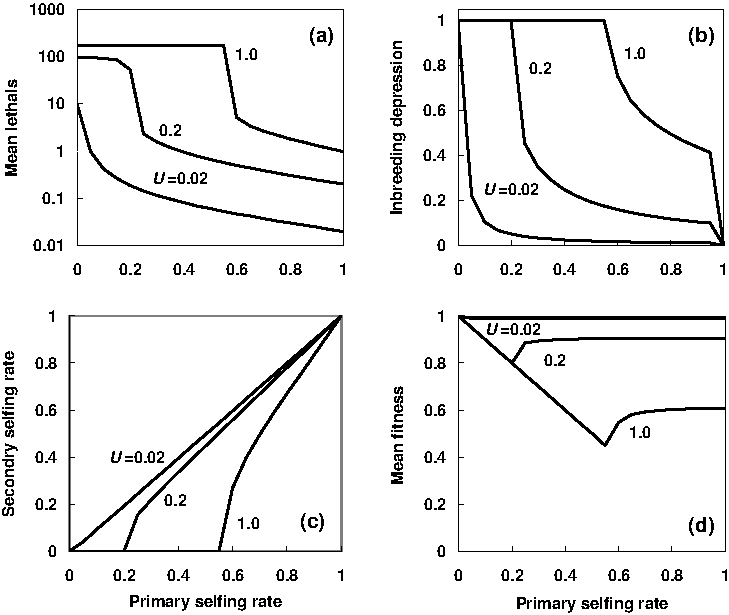
\includegraphics[height=4in,clip=]{k_lssh0_bb}

\caption[Recreation of \citet{Lande:1994:5345}, Figure~2]{Duplicate of the
results reported by \citet{Lande:1994:5345} in their Figure~2, for selection
coefficient $s=1.0$ and dominance $h=0.0$ at the given mutation rate and range
of selfing rates.  The sudden drop in inbreeding depression at a primary
selfing rate of 1 visible in panel (b) is an artifact of the method used to
compute inbreeding depression.  As is apparent in panel (d), this does not
reflect rapid changes in mean population fitness.}

\label{fig:k_lssh0}
\end{center}
\end{figure}

\begin{figure}
\begin{center}
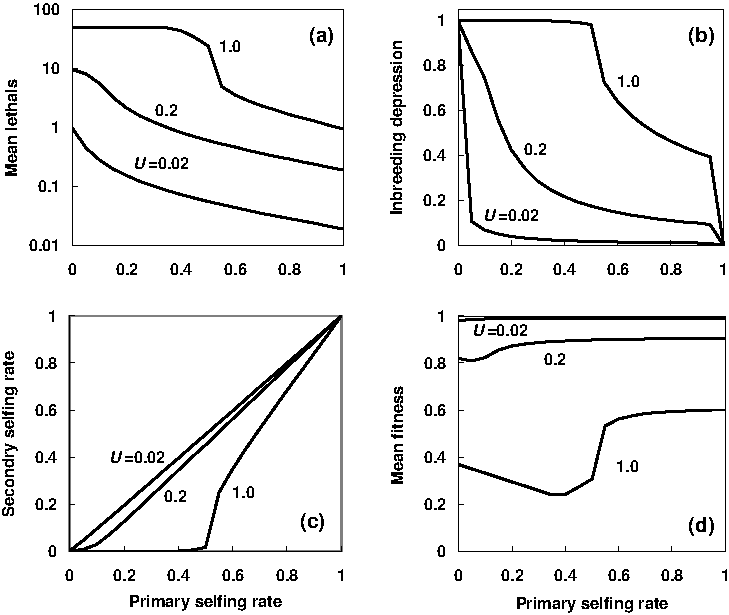
\includegraphics[height=4in,clip=]{k_lssh02_bb}

\caption[Recreation of \citet{Lande:1994:5345}, Figure~3]{Duplicate of the
results of \citet{Lande:1994:5345} in their Figure~3, for selection coefficient
$s=1.0$ and dominance $h=0.02$ at the given mutation rate and range of selfing
rates.  The same caution applies for panel (b) as in Figure~\ref{fig:k_lssh0}.}

\label{fig:k_lssh02}
\end{center}
\end{figure}

%%%%%%%%%%%%%%%%%%%%%%%%%%%%%%%%%%%%%%%%%%%%%%%%%%%%%%%%%%
%%%%%%%%%%%%%%%%%%%%%%%%%%%%%%%%%%%%%%%%%%%%%%%%%%%%%%%%%%
\chapter{Mutation}
\label{chapter:mutation}
%%%%%%%%%%%%%%%%%%%%%%%%%%%%%%%%%%%%%%%%%%%%%%%%%%%%%%%%%%
%%%%%%%%%%%%%%%%%%%%%%%%%%%%%%%%%%%%%%%%%%%%%%%%%%%%%%%%%%

In \K\ each new mutation is assumed to be unique.  Therefore, each new mutation
increases the number of heterozygous mutations in the population and does not
affect the number of homozygous mutations.  The mutation rate $U$ is
per-diploid genome, per-generation, and is taken to specify the mean of a
Poisson distribution \ProbDist{Poi}{U} specifying the distribution of the
number of new mutations {\cite[and many
others]{Kondrashov:1985:5375,Charlesworth:1990:5337}.  The proportion of load
class $L_{n,j}$ that is moved to load class \Lij\ (where $n \le i$) as a result
of mutation is equal to the probability that $i-n$ mutations occur, and is thus
the value of the $i-n$-th term of \ProbDist{Poi}{U}.  The total proportion of
the population in \xpijg\ after mutation is:

\begin{equation}\label{eq:mut:fullequation}
    \xpijg = 
    \begin{cases}
        \sum_{n \le i}{e^{-U} \frac{U^{i-n}}{(i-n)!} \cdot \xnjg} & U > 0 \\
        \xijg & U = 0
    \end{cases}
\end{equation}

There is currently no provision for specifying an alternative mutation function
as there is for fitness (section~\ref{section:definingfitnessfunction}).

%%%%%%%%%%%%%%%%%%%%%%%%%%%%%%%%%%%%%%%%%%%%%%%%%%%%%%%%%%
\section{Precomputed mutation terms}
\label{section:precomputedmutation}
%%%%%%%%%%%%%%%%%%%%%%%%%%%%%%%%%%%%%%%%%%%%%%%%%%%%%%%%%%

For computational efficiency, \K\ automatically calculates values for each term
$t\in(0,\Mi)$ of \ProbDist{Poi}{U}, where $t=i-n$ as in
equation~\eqref{eq:mut:fullequation}, and stores these values in the array
\lstinline{K->mut_term[t]}.  The function \lstinline{mut_term(K,t)} returns the
corresponding element of this array.

\sloppy Precomputed mutation values are established as a consequence of calling
the function \lstinline{initiate_model_state()} just prior to starting the
model.  The mutation rate \lstinline{K->U} must have the desired value prior to
this time.  The function \lstinline{mut_term_computed(K,x)} may be used to
bypass the precomputed values and calculate the mutation term directly.

%%%%%%%%%%%%%%%%%%%%%%%%%%%%%%%%%%%%%%%%%%%%%%%%%%%%%%%%%%
%%%%%%%%%%%%%%%%%%%%%%%%%%%%%%%%%%%%%%%%%%%%%%%%%%%%%%%%%%
\chapter{Reproduction}
\label{chapter:Kreproduction}
%%%%%%%%%%%%%%%%%%%%%%%%%%%%%%%%%%%%%%%%%%%%%%%%%%%%%%%%%%
%%%%%%%%%%%%%%%%%%%%%%%%%%%%%%%%%%%%%%%%%%%%%%%%%%%%%%%%%%

The structure of \K's modeling of reproduction reflects the independence of the
load class and genotype.  {\em Mating functions} define the result of different
types of matings for both load classes and functional genotypes.  The
membership in load classes following reproduction depends upon the mating
functions for load classes and functional genotypes involved, the population
rate of the mating system involved, and membership in load classes involved in
matings.

The mating functions for selfing and apomixis reflect the fact that just one
parental genotype is involved in the production of progeny.  The mating
functions for outcrossing, on the other hand, require two parental genotypes.

%%%%%%%%%%%%%%%%%%%%%%%%%%%%%%%%%%%%%%%%%%%%%%%%%%%%%%%%%%
\section{Load class mating functions}
%%%%%%%%%%%%%%%%%%%%%%%%%%%%%%%%%%%%%%%%%%%%%%%%%%%%%%%%%%

Load class mating functions for selfing and apomixis follow
\citet{Kondrashov:1985:5375}:

\begin{equation}
\label{eq:Kreproduction:s}
\funcself =
    \begin{cases}
        \binom{n}{i}\binom{n-i}{j-v}\cdot\left({\frac{1}{2}}\right)^{2n-i} & \text{$i\in(0,n)$, $j\in(v,v + n)$, $i+j \leq n+v$} \\
        0                                                                  & \text{otherwise.} 
    \end{cases}
\end{equation}
\begin{equation}
\label{eq:Kreproduction:a}
\funcapomixis = 
    \begin{cases}
        1  &  \text{$i=n$, $j=v$} \\
        0  &  \text{otherwise.}  
    \end{cases}
\end{equation}

For outcrossing, the modification of \citet{Charlesworth:1990:5337} is used, as
it is much more efficient than the function given in
\citet{Kondrashov:1985:5375}.  Note, though, that there are typographical
errors in \citeauthor{Charlesworth:1990:5337}'s Equation~(3).  This method
first forms pools of haploid male and female gametes, and the proportion of
available female gametes is weighted by the outcrossing rate.  A function for
production of gametes with functional genotypes is required, as is a function
for production of functional genotypes for zygotes formed from two genotyped
gametes:

\begin{align}
\label{eq:Kreproduction:gametes}
\gami    &= \begin{cases}
              \sum_{v=0}^{i}{
                \;  \sum_{n=i-v}^{M_i}{
                \binom{n}{i-v} \left(\frac{1}{2}\right)^{n} \xpnv
              }} & v \le \Mj \\
              0 & \text{otherwise}
            \end{cases} \\
\gamfemalei &= \Og \cdot \gami \\
\gammalei &= \gami
\end{align}

Zygotes are formed by matings among male and female gametes:

\begin{equation}
\label{eq:Kreproduction:zygotes}
\xppoig = \frac{1}{2} \sum_{k=0}^{i}{\gamfemalek\gammaleik+\gamfemaleik\gammalek}
\end{equation}

%%%%%%%%%%%%%%%%%%%%%%%%%%%%%%%%%%%%%%%%%%%%%%%%%%%%%%%%%%
\section{Genotype mating functions}
%%%%%%%%%%%%%%%%%%%%%%%%%%%%%%%%%%%%%%%%%%%%%%%%%%%%%%%%%%

The genotype mating functions shown in
Table~\ref{tab:matingK:stdtransformations} likewise follow
\citet{Kondrashov:1985:5375}.  For the outcrossed genotype mating function
\TOgab, the resulting genotype $\gamma_i$ is the Mendelian product of both
parents' genotypes.

The tables described here apply to genotypes determined by a single diploid
locus.  Alternative genotype mating functions may be easily defined that
determine these genotypes based on other assumptions (e.g., more than one
locus).

%%%%%% Standard transformations for genotypes
\begin{table}

\topcaption[Mating functions based upon perfect Mendelian segregation for
functional genotypes controlled by a single biallelic locus]{Mating functions
based upon perfect Mendelian segregation for functional genotypes controlled by
a single biallelic locus as described in the text.  Note that for \TSgx\ and
\TAgx\ each submatrix represents the resulting proportion of the progeny that
carry each functional genotype $(\gamma_1\ \gamma_2\ \gamma_3)$, and that the
proportions in each submatrix sum to $1$.}

\label{tab:matingK:stdtransformations}
\begin{center}
\begin{tabular}{c@{\extracolsep{0.5in}}cc}  % to set up a 1 x 3 array to display 3 tables
    % selfing - functional genotype mating function
    \begin{tabular}{c|c}
        \multicolumn{2}{c}{\TSgx}   \\
        \hline %-------------------------------
        $\xi_1$ & $(\begin{smallmatrix}1&0&0\end{smallmatrix})$ \\
        $\xi_2$ & $(\begin{smallmatrix}\frac{1}{4}&\frac{1}{2}&\frac{1}{4}\end{smallmatrix})$ \\
        $\xi_3$ & $(\begin{smallmatrix}0&0&1\end{smallmatrix})$
    \end{tabular}
    &  % end of leftmost table element
    % apomixis - functional genotype mating function
    \begin{tabular}{c|c}
        \multicolumn{2}{c}{\TAgx}   \\
        \hline %-------------------------------
        $\xi_1$ & $(\begin{smallmatrix}1&0&0\end{smallmatrix})$ \\
        $\xi_2$ & $(\begin{smallmatrix}0&1&0\end{smallmatrix})$ \\
        $\xi_3$ & $(\begin{smallmatrix}0&0&1\end{smallmatrix})$
    \end{tabular}
    &  % end of center tabular element
    % outcrossing - functional genotype mating function
    \begin{tabular}{c|cc}
        {\TOgab}    & $\beta_1$   & $\beta_2$ \\
        \hline %-------------------------------
        $\alpha_1$  & $\gamma_1$  & $\gamma_2$ \\
        $\alpha_2$  & $\gamma_2$  & $\gamma_3$
    \end{tabular}
    % end of rightmost tabular element
\end{tabular}
\end{center}
\end{table}

%%%%%%%%%%%%%%%%%%%%%%%%%%%%%%%%%%%%%%%%%%%%%%%%%%%%%%%%%%
\section{Net effect of mating}
%%%%%%%%%%%%%%%%%%%%%%%%%%%%%%%%%%%%%%%%%%%%%%%%%%%%%%%%%%

Note that each genotype $\gamma_i$ may have its own selfing, apomixis and
outcrossing rate $S(\gamma_i)$, $A(\gamma_i)$, and $O(\gamma_i)$, respectively.

%%%%%% Functions for determining total L(g;i,j) representation in matings of all genotype load classes
\begin{align}
\label{eq:Kreproduction:xppsijg}
\xppsijg &= 
    \sum_{n}{
		\sum_{v}{
		    \funcself \sum_{\xi}{\TSgx \cdot S(\xi) \cdot \xpijx}
		}
	}
\\
\label{eq:Kreproduction:xppaijg}
\xppaijg &= 
    \sum_{n}{
		\sum_{v}{
			\funcapomixis \sum_{\xi}{\TAgx \cdot A(\xi) \cdot \xpijx}
		}
	}
\\
\label{eq:Kreproduction:xppoijg}
\xppoijg &= 
    \sum_{n}{
		\sum_{v}{
			\sum_{l}{
				\sum_{m}{
					\funcoutcross 
					\sum_{\xi}{\sum_{\zeta}{\TOgab \cdot O(\xi) \cdot \xpijx}}
				}
			}
		}
	}
\end{align}

Total progeny frequencies are simply the sum of the proportions of selfed,
apomictic and outcrossed progeny:

\begin{equation}
\xppijg = 
\begin{cases}
    \xppoig + \xppsijg + \xppaijg  &  j=0               \\
    \xppsijg + \xppaijg            &  \text{otherwise}
\end{cases}
\end{equation}

%%%%%%%%%%%%%%%%%%%%%%%%%%%%%%%%%%%%%%%%%%%%%%%%%%%%%%%%%%
%%\subsection{Verifying mating functions within the model}
%%
%%Within \K\ source code, the function \Kcode{isOK\_repro\_transformations(K)} can be used at any time to ensure that these transformations are consistent.  The function quietly returns {\tt 1} if the transformations conform to Mendelian laws.  If any transformation is not consistent with Mendelian laws, the function produces output specifying any violations and returns {\tt 0}. 
%%%%%%%%%%%%%%%%%%%%%%%%%%%%%%%%%%%%%%%%%%%%%%%%%%%%%%%%%%

%\section{Examples}
%
%\subsection{Equilibrium distribution under outcrossing with no mutation}
%
%Using \K, we can see that the distribution of completely recessive heterozygous mutations at equilibrium in a completely outcrossing population with new new mutation is equivalent to the limiting case of the binomial distribution $\text{Bin}(\infty,p) \text{ where } p=\frac{\text{E}(i)}{\infty}$, which is equivalent to the Poisson distribution $\text{Poi}(\text{E}(i))$.  There is no mutation to create new mutations, and no selection to remove existing mutations.  The process producing the distribution is a binomial process involving an infinite number of loci, therefore it is reasonable that it should be equivalent to a Poisson distribution as it is the limiting case of the binomial distribution.  This may be implemented with the following code:
%
%\begin{C}[gobble=4]
%    set_repro_one_genotype(K, 0.0, 0.0, 0.0, 0.0);  /* outcrossing */
%    set_debug(DEBUG_DISABLEMUTATION);  /* turn off mutation */
%    fill_KArray(K, K->x, 0.0);  /* Every class is empty... */
%    K->x[10][0][0] = 1.0;  /* ... except for L(10,0;0) */
%    ... run model to equilibrium ...
%    dump_KArray(K, K->x);  /* View distribution at equilibrium */
%\end{C}

%%%%%%%%%%%%%%%%%%%%%%%%%%%%%%%%%%%%%%%%%%%%%%%%%%%%%%%%%%
%%%%%%%%%%%%%%%%%%%%%%%%%%%%%%%%%%%%%%%%%%%%%%%%%%%%%%%%%%
\chapter{Fitness}
%%%%%%%%%%%%%%%%%%%%%%%%%%%%%%%%%%%%%%%%%%%%%%%%%%%%%%%%%%
%%%%%%%%%%%%%%%%%%%%%%%%%%%%%%%%%%%%%%%%%%%%%%%%%%%%%%%%%%

In \K, just as in nature, selection reduces proportions of less fit genotypes.
Fitness in \K\ is typically a function of the mutations carried in the load
class \Lij, together with any user-specified parameters carried in the
\KConfig\ structure \KK.  In order to maintain the infinite population at
constant sum $1$, the application of selection reduces the proportions of load
classes below the population mean fitness and increases the proportions of load
classes above the population mean fitness.  Fitness may also be dependent upon
the genotype $\gamma$, but this has not typically been considered.


%%%%%%%%%%%%%%%%%%%%%%%%%%%%%%%%%%%%%%%%%%%%%%%%%%%%%%%%%%
\section{Specifying the fitness model}
%%%%%%%%%%%%%%%%%%%%%%%%%%%%%%%%%%%%%%%%%%%%%%%%%%%%%%%%%%

% A fitness function in \K\ returns a \KScalar.

\citet{Kondrashov:1985:5375} specified a fitness model that enabled threshold selection:
\begin{equation}\label{eqn:kondrashovfitness}
\omega_{i,j}=1-\left({\frac{1+dj}{k}}\right)^\alpha.
\end{equation}

The numbers of heterozygous and homozygous mutations are specified by $i$ and
$j$, respectively; individuals with $>k$ mutations died; $d$ specifies
dominance with $d=2$ equal to codominance; and $\alpha=1$, $2$, and $\infty$
correspond to linear, intermediate and threshold selection, respectively.

At the moment, \K\ does not provide Kondrashov's fitness function.  Instead, it
provides the familiar multiplicative fitness function parameterized by
selection coefficient $s\in(0,1)$ and dominance $h\in(0,1)$.  The fitness of a
given genotype is thus:

\begin{equation}\label{eq:fitnessmultiplicative}
\omega_{i,j}=(1-hs)^{i}(1-s)^{j}.
\end{equation}

Mean population fitness is determined by:

\begin{equation}\label{eq:meanfitness}
\bar{\omega}=\frac{\sum_i{\sum_j{\omega_{i,j}\xppij}}}{\sum_i{\sum_j{\xppij}}}
\end{equation}

and is returned by the function \lstinline{mean_fitness(K,K->xpp)}.

%%%%%%%%%%%%%%%%%%%%%%%%%%%%%%%%%%%%%%%%%%%%%%%%%%%%%%%%%%
\section{Precomputed fitness}
\label{section:precomputedfitness}
%%%%%%%%%%%%%%%%%%%%%%%%%%%%%%%%%%%%%%%%%%%%%%%%%%%%%%%%%%

For computational efficiency, \K\ automatically calculates fitnesses for all
\Lijg\ and stores these values in the array \lstinline{K->fitness_precomputed}.
The function\linebreak \lstinline{fitness(K,i,j,g)} returns the corresponding
element of this array.

Precomputed fitness values are established as a consequence of calling the
function \lstinline{initiate_model_state()} just prior to starting the model.
All relevant members of \KK\ must have values prior to this time.  The use of
precomputed fitness values is appropriate for the fitness functions supplied
with \K.  The function \lstinline{fitness_computed(K,i,j,g)} may be used to
bypass the precomputed values and calculate fitness directly.

If a fitness function is defined
(section~\ref{section:definingfitnessfunction}) that may determine different
fitness values for identical \Lijg\ at different times during model execution,
then it must be determined which of the following cases applies:

\begin{enumerate}
	\item\label{fitness:fewchanges} Fitness values may change one to several discrete times; or
	\item\label{fitness:manychanges} Fitness values may change many times. 
\end{enumerate}

If case (\ref{fitness:fewchanges}) fits, then points should be identified
during model execution at which precomputed values in
\lstinline{K->fitness_precomputed} should be recomputed.  At these times, all
relevant members of \KK\ should be updated, and then the function
\lstinline{initiate_fitness_precomputed()} is called.  The fitness function
itself may be changed at this time by changing the value of
\lstinline{K->fitness_function}:

\begin{C}[gobble=4,escapechar=|]
    if ( |{\it fitness values must change}| ) {
        /*
        ** First, change all relevant members of K (e.g., K->fit_s 
        ** and K->fit_h) and then recompute the values.
        */
        K->fit_s = 0.80;  /* decrease the selection coefficient */
        initiate_fitness_precomputed(K);
    }
\end{C}

If the fitness function instead fits case (\ref{fitness:manychanges}), then the
use of precomputed fitness values must be disabled by telling \K\ to directly
compute fitness every time a fitness value is required.  This is more
computationally intensive.  The use of precomputed fitness values is disabled
by calling the function \lstinline{must_compute_fitness_function()} and passing
the registered value of the fitness function (which was stored in
\lstinline{K->fitness_function)} as the sole argument:

\begin{C}[gobble=4]
    /* Force computation of fitness every time */
    must_compute_fitness_function(K->fitness_function);
\end{C}

After doing this, the function \lstinline{fitness(K,i,j,g)} is operationally
identical to the function \lstinline{fitness_computed(K,i,j,g)}.  There is
currently no mechanism to return to precomputed fitness values once
\lstinline{must_compute_fitness_function()} has been called.

%%%%%%%%%%%%%%%%%%%%%%%%%%%%%%%%%%%%%%%%%%%%%%%%%%%%%%%%%%
\section{Defining a new fitness function\label{section:definingfitnessfunction}}

In \K, fitness functions share a common interface.  The first argument is
always the active \KConfig\ \KK, the second and third arguments are both \KInt\
and specify the number of heterozygous and homozygous mutations, respectively,
in the load class of interest, and the fourth argument specifies the genotype
of interest and is also \KInt.  Once the fitness value is computed from the
load class and genotype arguments together with any parameters from \KConfig\
\KK, the fitness value returned as a \KScalar.

Because fitness functions share a common interface, a new fitness function may
be easily defined and incorporated into \K.  Within the body of the fitness
function, fitness is calculated using the load class and genotype arguments
along with any members of \KK\ (e.g.\ \lstinline{K->fit_s} and
\lstinline{K->fit_h}) that are being used as parameters.  The fitness is
computed as a \KScalar\ and returned as the function value:

\begin{C}[gobble=4,mathescape=true,escapechar=|]
    KScalar  newfitnessfunction  (KConfig K, KInt i, KInt j, KInt g)
    {
        KScalar w;       /* w will hold the computed fitness */
        KScalar t1, t2;  /* intermediate values */
        /*
        ** The example fitness function is the multiplicative
        ** fitness function |$w_{i,j}=(1-hs)^{i}(1-s)^{j}$|.
        **
        ** The C function pow(a,b) computes |$a^b$|.
        */
        t1 = pow((1 - K->fit_h*K->fit_s), i);
        t2 = pow((1 - K->fit_s), j);
        w = t1 * t2;
        return w;
    }
\end{C}

In order to use a new fitness function it must be registered.  This is done
prior to the start of the model run, generally within \lstinline{main()}.  In
the declarations section the new fitness function is described with a {\em
function prototype}.  A function prototype is identical to the first line of
the function definition, but does not have a function body and ends with a
semicolon `\lstinline{;}'.  All fitness function prototypes will be identical
except for the name of the function.  Prior to use, a new fitness function is
registered by calling the function \lstinline{register_fitness_function()}.
This function requires two arguments: the name of the new fitness function
without parentheses, and a short character-string description.  \K\ uses the
new fitness function once the value returned by
\lstinline{register_fitness_function()} is assigned to
\lstinline{K->fitness_function}.  Any members of \KK\ used by the new fitness
function, e.g.\  \lstinline{K->fit_s}, must have values assigned prior to model
execution:

\begin{C}[gobble=4,escapechar=|]
    /* Function prototype for new fitness function within declarations */
    KScalar  newfitnessfunction  (KConfig K, KInt i, KInt j, KInt g);
    |{\it ... intervening code ...}|
    /* Register the fitness function */
    K->fitness_function = register_fitness_function(newfitnessfunction,
                                                    "new multiplicative");
    /* Set the members of K that are used by newfitnessfunction() */
    K->fit_s = 0.95;  /* E.g., highly recessive sublethal mutations*/
    K->fit_h = 0.02;
    |{\it ... continue with model loop ...}|
\end{C}


%%%%%%%%%%%%%%%%%%%%%%%%%%%%%%%%%%%%%%%%%%%%%%%%%%%%%%%%%%
%%%%%%%%%%%%%%%%%%%%%%%%%%%%%%%%%%%%%%%%%%%%%%%%%%%%%%%%%%
\chapter{Using nested mutation classes}
\label{chapter:nested}
%%%%%%

\K\ provides the ability to simultaneously examine the consequences of the
number of mutation classes $N_c > 1$ via {\em nesting}.  No published model has
yet made use of this feature \citetext{but see Scofield, unpubl.}, and the
extensions described here are entirely novel to \K.  As a result, this portion
of \K\ has not been adequately tested.

Space and execution time with nesting scale at approximately \Order{[{reqs.\ of
N_1}]^{N_c}}.  We will consider the case where $N_c = 2$, which represents a
squaring of space and time requirements.  We make two further simplifications.
We will consider load classes only, not genotypes, and we will also lose some
generality in the functions used for computing fitness.  Interested users may
extend \K's implementation of nested mutation classes by following the examples
given here and elsewhere in this document.

Each mutation class $c$ has its own mutation rate $U_c$, fitness function, and
fitness coefficients.  Load classes are called \emph{nested load classes} and
are represented by \Lijij, where $\izero\in(0,\Mizero)$ and
$\jzero\in(0,\Mjzero)$ represent the number of heterozygous and homozygous
mutations in the first mutation class and $\ione\in(0,\Mione)$ and
$\jone\in(0,\Mjone)$ represent the number of heterozygous and homozygous
mutations in the second mutation class.  The total number of nested load
classes is $(\Mizero+1)(\Mjzero+1)(\Mione+1)(\Mjone+1)$.  Model operations are
based upon the joint probability distribution of independent events in each
mutation class, thus the probability of a mutation event, a reproduction event,
etc.\ affecting \Lijij\ is the probability of the required events affecting
each mutation class individually:

\begin{equation}
Pr[\text{event in }\Lijij] = Pr[\text{event in }\Lijzero]\times Pr[\text{event in }\Lijone].
\end{equation}

%%%%%%%%%%%%%%%%%%%%%%%%%%%%%%%%%%%%%%%%%%%%%%%%%%%%%%%%%%
\section{Mutation in nested models}

As in an unnested model, mutation increases the number of heterozygous
mutations in the population and does not affect the number of homozygous
mutations.  The mutation process for each mutation class $c$ is equivalent to
the single-class process described in Chapter~\ref{chapter:mutation} determined
by \ProbDist{Poi}{U_c}, thus mutation increases the population proportion in
\Lijij\ at the expense of all $L(\nzero,\jzero,\none,\jone)$ where
$\nzero\le\izero$ and $\none\le\ione$.  The total proportion of the population
in \xpijij\ after mutation is thus:

\begin{equation}\label{eq:nested:fullequation}
    \xpijij = \sum_{n_0=0}^{i_0}{\; \sum_{n_1=0}^{i_1}{x_{n_0,j_0,n_1,j_1} \cdot e^{-U_0} \frac{U_0^{[i_0-n_0]}}{(\izero-\nzero)!} \cdot e^{-U_1} \frac{U_1^{[i_1-n_1]}}{(\ione-\none)!}}}
\end{equation}

If $U_c=0$ then the corresponding term of \ProbDist{Poi}{U_c} is replaced with
$1$ if $i_c-n_c=0$ and $0$ otherwise.

%%%%%%%%%%%%%%%%%%%%%%%%%%%%%%%%%%%%%%%%%%%%%%%%%%%%%%%%%%
\section{Reproduction in nested models}

As for mutation, reproduction in an nested model is a straightforward extension
of the unnested model.  Because mutation classes are independent, results for
each genotype are determined as the product of results for each mutation class.
Reproduction is by far the most time-consuming step in a nested model, so
judicious implementation of the qualifying conditions on indices appended to
each equation may speed execution by an order of magnitude or more:

\begin{equation}
\label{eq:nested:s}
\begin{split}
  \funcselfnested &= \binom{n_0}{i_0}\binom{n_0-i_0}{j_0-v_0}\binom{n_1}{i_1}\binom{n_1-i_1}{j_1-v_1}\left({\frac{1}{2}}\right)^{2(n_0+n_1)-i_0-i_1} ; \\
  & \qquad i_0\in(0,n_0),\;j_0\in(v_0,v_0 + n_0),\;i_0+j_0 \leq n_0+v_0,\\
  & \qquad i_1\in(0,n_1),\;j_1\in(v_1,v_1 + n_1),\;i_1+j_1 \leq n_1+v_1 
\end{split}
\end{equation}

\begin{equation}
\label{eq:nested:a}
\funcapomixisnested = 
  \begin{cases}
    1 & \text{$i_0=n_0$, $j_0=v_0$, $i_1=n_1$, $j_1=v_1$} \\
    0 & \text{otherwise.}  
  \end{cases}
\end{equation}

Haploid gametes carry one copy of mutations from each mutation class.  As for
the unnested model, the proportion of available female gametes is weighted by
the outcrossing rate:

\begin{align}
\begin{split}
\gamii   &= \sum_{v_0=0}^{i_0}{
	  						\; \sum_{v_1=0}^{i_1}{
                	\; \sum_{n_0=i_0-v_0}^{M_{i_0}}{
                		\; \sum_{n_1=i_1-v_1}^{M_{i_1}}{
                      \binom{n_0}{i_0-v_0} \binom{n_1}{i_1-v_1}
                      \left(\frac{1}{2}\right)^{n_0+n_1} \xpnvnv 
              }}}} ; \\ 
              & \quad v_0 \le \Mjzero, \; v_1 \le \Mjone
\end{split} \\
\gamfemaleii &= O \cdot \gamii \\
\gammaleii &= \gamii
\end{align}

Outcrossed zygotes are formed by matings among male and female gametes:

\begin{equation}
\label{eq:nested:zygotes}
\begin{split}
\xppoii &= 
  \frac{1}{4}
    \sum_{k_0=0}^{i_0}{} \;
      \sum_{k_1=0}^{i_1}{}
        \gamfemalekk\gammaleikik + \gamfemalekik\gammaleikk + \\
    &   \qquad\qquad\qquad\quad \gamfemaleikk\gammalekik + \gamfemaleikik\gammalekk.
\end{split}
\end{equation}

Adding up all progeny proportions gives:

\begin{equation}
\xppijij = 
\begin{cases}
\xppoii + \xppsijij + \xppaijij  & j_0=0,\;j_1=0 \\
\xppsijij + \xppaijij            & \text{otherwise}
\end{cases}
\end{equation}

%%%%%%%%%%%%%%%%%%%%%%%%%%%%%%%%%%%%%%%%%%%%%%%%%%%%%%%%%%
\section{Fitness and selection in nested models}

Fitness is determined for each mutation class as for an unnested model, and the
fitness of a nested load class is the product of the fitness functions of the
two mutation classes:

\begin{equation}
\wnested = \omega_{i_0,j_0} \cdot \omega_{i_1,j_1}.
\end{equation}

For example, if a multiplicative fitness model is used for each mutation class
then each mutation class has its own selection coefficient and dominance:

\begin{equation}
\wnested = (1-h_0 s_0)^{i_0}(1-s_0)^{j_0} \cdot (1-h_1 s_1)^{i_1}(1-s_1)^{j_1}.
\end{equation}

The computation of \wnested\ is a consequence of setting the fitness functions
for the mutation classes; no more need be done by the user.  The computation of
mean fitness with nested load classes \meanwnested\ is a straightforward
extension of Equation~\eqref{eq:meanfitness}:

\begin{equation}\label{eq:meanfitnessnested}
\meanwnested = \frac{\sum_{i_0}{\sum_{j_0}{\sum_{i_1}{\sum_{j_1}{\wnested\cdot\xppijij}}}}}
               {\sum_{i_0}{\sum_{j_0}{\sum_{i_1}{\sum_{j_1}{\xppijij}}}}}.
\end{equation}

This value is returned by the function \lstinline{mean_fitness_n()}.

Fitness values are precomputed for each mutation class $c$\/ prior to the start
of the model (see section~\ref{section:precomputedfitness}) and kept in the
array \lstinline[language=C]{KN->fitness_precomputed[c][i][j]}.  The function
\lstinline{fitness_n(KN,i0,j0,i1,j1)} uses this array to determine the fitness
of the nested load class \Lijij.  Fitness values may be computed directly via
\lstinline{fitness_computed_n()}.  Similar to unnested models, precomputed
fitness values can be recomputed with
\lstinline{initiate_fitness_precomputed_n()}; a call to this function will
recompute fitness values for both mutation classes.  Direct computation of
fitness values for each mutation class individually can be specified with
\lstinline{must_compute_fitness_function_n()}.

Selection is applied as for an unnested model:

\begin{equation}\label{eq:selectionnested}
\Xijij = \frac{\wnested\cdot\xppijij}{\meanwnested}
\end{equation}

%%%%%%%%%%%%%%%%%%%%%%%%%%%%%%%%%%%%%%%%%%%%%%%%%%%%%%%%%%
\section{Data structures for a nested model}

The basic structure of the nested model's data structures is very similar to
the unnested model.  The load class array names are all identical, with a
change in array shape to accommodate the nested load class \Lijij\ and the lack
of genotype, e.g., \lstinline{KN->x[i0][j0][i1][j1]} and
\lstinline{KN->xpp[i0][j0][i1][j1]}.  Most functions and datatypes used in a
nested model are special versions named by adding the suffix
``\lstinline{_n}''. 

The datatype \KConfign\ holds the parameters and data structures used in a
nested model, and references to this datatype within \K\ use the name \KKN.
Changes from the \KConfig\ datatype used in unnested models reflect both the
greater complexity of nested models and the simplified set of model options.
Real-valued parameters that differ between mutation classes are of the
\lstinline{KScalar_n} datatype, which is an array of \lstinline{KScalar}
values, one per mutation class.  For example, in a nested model the mutation
rate is modified using \lstinline{KN->U[0] = value0} for the zeroth mutation
class and \lstinline{KN->U[1] = value1} for the first.

%%%%%%%%%%%%%%%%%%%%%%%%%%%%%%%%%%%%%%%%%%%%%%%%%%%%%%%%%%
\section{Initiating and running a nested model}

The initiation of a \K\ session with nested mutation classes looks very much
like that for one mutation class.   except for the use of the \KConfign\
structure and the functions used are all special versions named by adding the
suffix ``\lstinline{_n}''.  Also, all values $U_c$, $s_c$, etc.\ that are
distinct between load classes are vectors declared as \lstinline{KScalar_n} or
\lstinline{KInt_n}.

\begin{C}[gobble=4]
    KConfig_n KN;
    KN = initiate_KConfig_n();
    initiate_load_classes_n(KN, MI0, MJ0, MI1, MJ1);
    KN->U[0] = 0.1;
    KN->U[1] = 0.9;
    KN->fitness_function[0] = FITNESS_MULTIPLICATIVE_n;
    KN->fitness_function[1] = FITNESS_MULTIPLICATIVE_n;
    KN->fit_s[0] = 1.0;  /* zeroth mut class highly recessive lethals */
    KN->fit_h[0] = 0.02;
    KN->fit_s[1] = 0.1;  /* first mut class more dominant & mild */
    KN->fit_h[1] = 0.3;
    KN->S = 0.0;
    set_repro_n(KN, KN->S, 0.0);
    initiate_model_state_n(KN);
\end{C}

As for model initiation, running a \K\ session with nested mutation classes
looks very much like that for one mutation class, except the
\lstinline{KConfig} structure and the functions used are all special versions
named by adding the suffix ``\lstinline{_n}''.

\begin{C}[gobble=4]
    compute_adults_initial_n(KN);
    while (! is_equilibrium_n(KN)) {
        if (KN->generation > GENERATION_CUTOFF_n)
            break;
        if (KN->option_truncate)
            truncate_KArray_n(KN, KN->x, LOADCLASS_TRUNCATE);
        compute_mutation_n(KN);
        compute_self_progeny_n(KN);
        compute_apomixis_progeny_n(KN);
        compute_gametes_n(KN);
        compute_zygotes_n(KN);
        compute_summed_progeny_n(KN);
        compute_fitness_n(KN);
        compute_adults_nextgen_n(KN);
        normalize_KArray_n(KN, KN->x);
    }
    stats_all_n(KN);
    stats_print_n(KN);
\end{C}


%%%%%%%%%%%%%%%%%%%%%%%%%%%%%%%%%%%%%%%%%%%%%%%%%%%%%%%%%%
%%%%%%%%%%%%%%%%%%%%%%%%%%%%%%%%%%%%%%%%%%%%%%%%%%%%%%%%%%
%%%%%%%%%%%%%%%%%%%%%%%%%%%%%%%%%%%%%%%%%%%%%%%%%%%%%%%%%%
%%%%%%%%%%%%%%%%%%%%%%%%%%%%%%%%%%%%%%%%%%%%%%%%%%%%%%%%%%
\chapter{Model parameters in \K}

Model parameters as used in \K\ and in Kondrashov (1985).  \dag\/Kondrashov did
not model the coexistence selfing and apomixis, and used the same parameter
names for the rate and discount of each.

\begin{landscape}

\label{tab:modelparameters}
\begin{longtable}{p{2in}|c|c|c|l}
\caption{Model parameters in \K} \\
Model Parameter			        &	\K              	&	Kondrashov		& Value modified & \K\ source code       \\ \hline
\endfirsthead
\caption{Model parameters in \K\ (continued)} \\
Model Parameter			        &	\K              	&	Kondrashov		& Value modified & \K\ source code       \\ \hline
\endhead
Genotype designation	      & $g, \xi, \zeta$	& $\kappa, \xi, \zeta$	& various & {\tt g}, {\tt gg}, {\tt xi}, {\tt zeta}, {\em etc.} \\
Selfing rate								& \Sg							& $z_\kappa$		& model start &	\Kmemberi{S}{genotype}   \\
Pollen discount to selfing	& \DSg						& $y_\kappa$		& model start &  \Kmemberi{D\_S}{genotype} \\
apomixis rate								& \Ag							& $z_\kappa$\dag 	&	model start & \Kmemberi{A}{genotype}   \\
Pollen discount to apomixis	& \DAg						& $y_\kappa$\dag	& model start & \Kmemberi{D\_A}{genotype} \\
Outcrossing rate						& \Og							& not named   	&	model start &	\Kmemberi{O}{genotype} \\
Resources for selfed ovules & \RSOg           & not named			& model start &	\Kmemberi{rsrc\_SO}{genotype} \\
Resources for apomictic ovules & \RAOg        & not named			& model start &	\Kmemberi{rsrc\_AO}{genotype} \\
Resources for outcrossed ovules & \ROOg       & not named			& model start &	\Kmemberi{rsrc\_OO}{genotype} \\
Resources for outcrossed pollen & \ROPg       & not named			& model start &	\Kmemberi{rsrc\_OP}{genotype} \\
Total resources used for ovules	& \Ffemale				&	\Ffemale			& each generation & \Kmember{F\_female} \\
Total resources used for pollen	& \Fmale					&	\Fmale				& each generation & \Kmember{F\_male} \\
Proportion of \Ffemale\ resources used for \Lij\ selfed ovules	&	\gammaij	&	\gammaij			& each generation & \Kmemberij{gamma}{i}{j} \\
Proportion of \Ffemale\ resources used for \Lij\ apomictic ovules	&	\alphaij	&	\alphaij	& each generation & \Kmemberij{alpha}{i}{j} \\
Proportion of \Ffemale\ resources used for \Lij\ outcross ovules	&	\betaij	&	\betaij				& each generation & \Kmemberij{beta}{i}{j} \\
Proportion of \Fmale\ resources used for \Lij\ outcross pollen	&	\rhoij	&	\rhoij				& each generation & \Kmemberij{rho}{i}{j} \\
Proportion of \gammaij\ used for \Lgij\ selfed ovules &	\SOijg	&	$a_{i,j}(\kappa)$\dag	& each generation & \Kmemberijk{SO}{genotype}{i}{j} \\
Proportion of \alphaij\ used for \Lgij\ apomictic ovules &	\AOijg	&	$a_{i,j}(\kappa)$\dag	& each generation & \Kmemberijk{AO}{genotype}{i}{j} \\
Proportion of \betaij\ used for \Lgij\ outcross ovules &	\OOijg	&	$g_{i,j}(\kappa)$	& each generation & \Kmemberijk{OO}{genotype}{i}{j} \\
Proportion of \rhoij\ used for \Lgij\ outcross pollen &	\OPijg	&	$h_{i,j}(\kappa)$	& each generation & \Kmemberijk{OP}{genotype}{i}{j} \\
\end{longtable}

\end{landscape}

Note to Doug: consider sorting this table by parameter name, and changing the columns around.  Also note the typesetting disaster that is the table caption.

%%%%%%%%%%%%%%%%%%%%%%%%%%%%%%%%%%%%%%%%%%%%%%%%%%%%%%%%%%
%%%%%%
\chapter{Debugging Guide for \K}
%%%%%%

\REDO\  \K\ is a complex system, and as such it is only to be expected that
modifications or new implementations of model portions will have bugs that will
need to be found and corrected.  This chapter is a guide to resolving these
problems and to the facilities provided within \K\ to assist in resolving these
problems.

\section{Reproduction}

\subsection{Diagnostics relevant to problems with reproduction}

\subsection{Progeny proportions}

If the integrity of functions described in Chapter~\ref{chapter:Kreproduction}
for determining \Lijg\ of progeny resulting from matings, then variation in
load class genotypes may be unnecessarily complicating the diagnosis of the
problem.  It would be better to start with a highly simplified adult \Lijg\ to
reduce the load classes of progeny that can be produced.  The first step is to
disable the mutation process.  This can be done by either commenting out
references to the function \lstinline{compute_mutation(K)} or by specifying the
diagnostic switch \lstinline{DEBUG_DISABLE_MUTATION} (see subsection~[whatever]
for the specification of diagnostic switches).  Then, new adult load classes
must be specified.  First, use \lstinline{fill_KArray(K,K->x,0.0)} to set all
adult \Lijg\ to zero.  Then, specify \Lijg\ proportions that may help to
resolve the problem.  For example, to examine what appears to be a basic
problem with \lstinline{o_outcross()}, place all adults in load class
\LCG{1}{0}{0} with \lstinline{K->x[1][0][0]=1.0}.  Then execute the model and
examine \Lijg\ of progeny produced.

Remember that the sum of adult \Lijg\ must equal \lstinline{1} prior to
reproduction; this can be verified by checking that
\lstinline{(sum_KArray(K,K->x)==1.0)} or by specifying the diagnostic switch
\lstinline{DEBUG_NORMALIZATION}.

\section{Decreasing execution time}

There are two important rules to consider before attempting to decrease the
execution time of a computer program:

\begin{enumerate}
	\item \label{ruletoomuch} Be sure that the program is actually taking too much time, by your own definition.  If so, then ...
	\item \label{rulefocus} Only work on those parts of the program that actually use a lot of time.
\end{enumerate}

If you don't follow these rules, you may find that you've either been trying to
improve an already fast program, or that you've been making only minor
improvements to a slow program.  If Rule~\ref{ruletoomuch} applies, first try
compiling \K\ with compiler optimization turned on.  In Visual Studio on
Windows, select the release build configuration via '\Cmdline{Build > Set
Active Configuration ... > Win32 Release}'.  On Unix/Linux, type '\Cmdline{make
opt}' or add the \Cmdline{-O3} option while compiling.

If Rule~\ref{ruletoomuch} still applies after optimized compilation, then you
can apply Rule~\ref{rulefocus} by identifying functions that take too much
time.  In Visual Studio on Windows, I have no idea how to do this.  On
Unix/Linux systems, the \Cmdline{gprof} utility will tell you exactly the
information you require.  Type '\Cmdline{man gprof}' at a shell prompt for more
information.

Once you've identified functions that are too slow, first consider algorithmic
improvements.  For example, the generation of outcross offspring via
\citeauthor{Kondrashov:1985:5375}'s \citeyearpar{Kondrashov:1985:5375} function
requires \Order{M_i^3 \times M_j^2} time to execute.  By modifying the
outcrossing process to first produce gametes \Order{M_i^2 \times M_j} and then
zygotes \Order{M_i^2} as did \citet{Charlesworth:1990:5337}, an increase in
speed was obtained.

%%%%%%%%%%%%%%%%%%%%%%%%%%%%%%%%%%%%%%%%%%%%%%%%%%%%%%%%%%
%%%%%%
\chapter{Source code conventions for \K}
%%%%%%

\begin{C}[aboveskip=\bigskipamount,caption={\K\ function template},label=K:sourcecode:functiontemplate]
/*///////////////////////////////////////////////////////////////*/
KScalar     my_function         (KConfig K, KArray arg1, KInt arg2);
{
    const char* thisfunction = "my_function";
    /* ... the rest of the function ... */
}
\end{C}

%%%%%%%%%%%%%%%%%%%%%%%%%%%%%%%%%%%%%%%%%%%%%%%%%%%%%%%%%%
%%%%%%%%%%%%%%%%%%%%%%%%%%%%%%%%%%%%%%%%%%%%%%%%%%%%%%%%%%
\bibliography{K_manual}
%%%%%%%%%%%%%%%%%%%%%%%%%%%%%%%%%%%%%%%%%%%%%%%%%%%%%%%%%%
%%%%%%%%%%%%%%%%%%%%%%%%%%%%%%%%%%%%%%%%%%%%%%%%%%%%%%%%%%

%%%%%%%%%%%%%%%%%%%%%%%%%%%%%%%%%%%%%%%%%%%%%%%%%%%%%%%%%%
%%%%%%%%%%%%%%%%%%%%%%%%%%%%%%%%%%%%%%%%%%%%%%%%%%%%%%%%%%
\end{document}
%%%%%%%%%%%%%%%%%%%%%%%%%%%%%%%%%%%%%%%%%%%%%%%%%%%%%%%%%%
%%%%%%%%%%%%%%%%%%%%%%%%%%%%%%%%%%%%%%%%%%%%%%%%%%%%%%%%%%

